\section{Freifunk}
\subsection{Was ist Freifunk?}
Im Zeitalter der Digitalisierung sind wir immer und überall vernetzt, doch lassen wir das Netz von anderen betreiben und machen uns so von diesen wenigen Betreibern abhängig. Freifunk ist eine Initiative, die den Aufbau eines Netzes in die eigene Hand nimmt und so jedem ermöglicht, ein vollwertiger und wichtiger Teil des Netzwerks zu werden. Hierfür bauen wir ein stadtweites drahtloses Netzwerk auf. Dabei entsteht ein Mesh-Netzwerk mit vielen Knotenpunken, über die die Daten fließen. Diese Knoten sind Freifunk-Router (also Router, wie du sie von zuhause kennst mit einer speziellen Software, der Freifunk-Firmware), die miteinander über WLAN-Technologie kommunizieren und die Daten untereinander austauschen. Außerdem stellt jeder von ihnen zeitgleich einen offenen Zugangspunkt in dieses Netz zur Verfügung, mit dem man sich mit Handy, Notebook oder Tablet einfach verbinden kann. So kannst du neben den internen Diensten auch auf das Internet zugreifen und zum Beispiel dein Mobilfunkvolumen sparen. Natürlich kannst du auch selbst Dienste anbieten, die dann jedem in Fulda zur Verfügung stehen, sobald er sich mit dem Netzwerk verbindet.

\subsection{Wie funktioniert Freifunk?}
Freifunk wird von einer Gruppe von Freiwilligen in Gemeinschaftsarbeit gepflegt. Die Freifunk-Community sorgt dafür, dass auch hinter den Knoten alles funktioniert, pflegt und erweitert die Software für die Knoten, stellt Freifunk auf öffentlichen Veranstaltungen vor, organisiert den Ausbau oder redet einfach nur mit den Nachbarn über Freifunk. An der technischen Arbeit kann man sich beteiligen, muss man aber nicht.
Technisch gesehen bauen die Freifunk-Knoten ein sogenanntes Mesh-Netzwerk untereinander auf. Das funktioniert immer, wenn sich zwei Knoten gegenseitig empfangen. Wie weit die Knoten senden und in welchem Umkreis sie andere Knoten empfangen können, liegt am Typ und den verwendeten Antennen. Damit die dabei entstehenden Mesh-Wolken sich auch über große Distanzen erreichen können und das Netzwerk überhaupt vollständig funktioniert, kann jeder Knoten einen Teil der Bandbreite seines Internetanschlusses teilen, um die Freifunk-Gateway-Server zu erreichen. So bildet sich über diese Tunnelverbindungen eine große Mesh-Wolke, über die die Daten übermittelt werden.

\subsection{Wie kann ich am Freifunk mitmachen?}

Um selbst Freifunk zu betreiben und somit Teil des großen Ganzen zu werden, brauchst du nichts weiter als einen kleinen WLAN Router, den du bei dir zu Hause aufstellst und mit dem Internet oder anderen Freifunkknoten verbindest. Durch eine spezielle Software wird dieses Gerät dann ein sogenannter Freifunk Knoten.
Wie genau das funktioniert und welche anderen Möglichkeiten es gibt um mitzumachen, findest du in unserer Mitmachen-Sektion.

\newpage
\begin{textblock*}{30mm}(165mm,5mm)
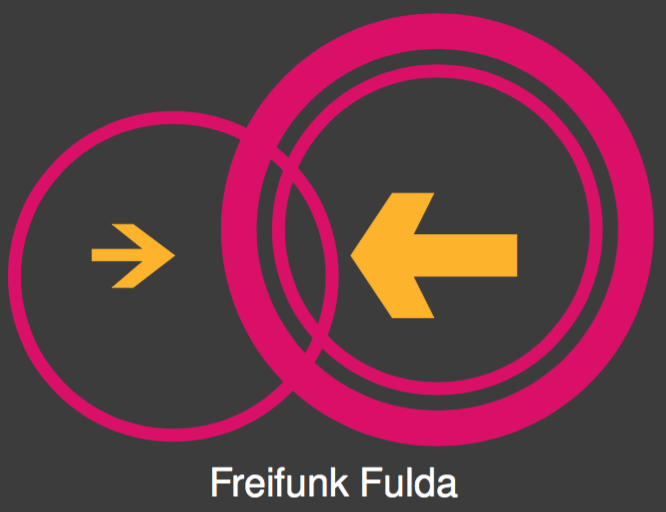
\includegraphics[height=30mm,width=39mm]{./FFLogo.png}\\
% \color{white}
\end{textblock*}
\subsection{Warum wird Freifunk gebraucht?}

Die Möglichkeit, Informationen immer und überall zu erhalten und mit anderen zu teilen, ist heutzutage elementarer Bestandteil unseres täglichen Lebens. Lange Zeit wurde das Internet und alles, was damit zu tun hat, von politischer Seite nicht wichtig genommen. Das hat dazu geführt, dass die elektronische Kommunikation heute in wesentlichen Teilen der demokratischen Kontrolle entzogen ist und in den Händen weniger großer Telekommunikationskonzerne liegt. Hier setzt der Gedanke von Freifunk an und möchte eine Alternative bieten: für jeden frei zugängliches Internet, ohne dafür zahlen zu müssen. Darum geht es bei Freifunk: dass alle Menschen an der Gemeinschaft teilhaben können – nicht mehr und nicht weniger.